%****************************************************************************
% Title     : Manuel utilisateur
% Author    : SEEMULLER Julien
% Date      : 2016-2017
% Version   : 1.0
%****************************************************************************

\documentclass[a4paper, french]{article}
\usepackage[utf8]{inputenc}
\usepackage{babel}
\usepackage{csquotes}
\usepackage[T1]{fontenc}
\usepackage[left=2.5cm,right=2.5cm,top=3cm,bottom=3cm]{geometry}
\usepackage{graphicx}
\usepackage{calc}
\usepackage{enumitem}
\usepackage{framed}
\usepackage[linktoc=all]{hyperref}
\usepackage{fancyhdr}
\usepackage{layout}
\usepackage[dvipsnames]{xcolor}
\usepackage{listings}
\usepackage{pdfescape}
\usepackage{wrapfig}
\usepackage{pdflscape}
\usepackage{rotating}
\usepackage{epstopdf}
\usepackage{xstring}
\usepackage{lastpage}
\usepackage{tikz}
\usepackage{pgfgantt}
\usepackage{csquotes}
\usepackage{dirtree}
\usepackage{fontawesome}
\usepackage[backend=biber, style=numeric, sorting=none]{biblatex}
 
% Command to make circled numbers
\newcommand*\circled[1]{\tikz[baseline=(char.base)]{
                \node[shape=circle,thick,draw,inner sep=2pt] (char) {\textbf{#1}};}
            }

\newcommand*\tinycircled[1]{\tikz[baseline=(char.base)]{
                \node[shape=circle,draw,inner sep=1pt] (char) {\footnotesize{#1}};}
            }

\addbibresource{references.bib} 

\lstloadaspects{formats}
\graphicspath{{img/}}


% Configure hyperref
\hypersetup{
    colorlinks,
    citecolor=black,
    filecolor=black,
    linkcolor=black,
    urlcolor=blue
}

% Set the docs variables
\title{Prisoner's Dilemma Cellular Automaton}
\newcommand{\subtitle}{Manuel Utilisateur}
\author{\textsc{Julien SEEMULLER}}
\date{\today}
\newcommand{\lesson}{Travaux de Diplômes 2017}
\newcommand{\class}{T.IS-E2B}
\newcommand{\teacher}{Mme. Terrier}

% Save the values
\makeatletter
 
 % Header and footers
\pagestyle{fancy}
\fancyhf{}
\lhead{\@title}
\rhead{\class}
\lfoot{\lesson}
\rfoot{Page \thepage{} / \pageref{LastPage}}

% Header and footer lines
\renewcommand{\headrulewidth}{1pt}
\renewcommand{\footrulewidth}{1pt}

% Spacing params
\setlength\parindent{0pt}
\setlength{\parskip}{0.75em}

\setcounter{tocdepth}{3}

\begin{document}
% Title page
\begin{titlepage}
	\centering
	{\scshape\LARGE CFPT-INFORMATIQUE \par}
	\vspace{0.25cm}
	{\scshape\lesson\par}
	\vspace{3cm}
	
	\hrule
	{\huge\bfseries\textsc\@title\par}
	{\Large\bfseries\textsc\subtitle\par}
	\vspace{0.5cm}
	{\itshape\@author\par}
	\vspace{1cm}
	{\textit{Supervisé par :}  \par \textsc{\teacher}}\par
	\vspace{0.5cm}
	\hrule
	
	\vfill
	
\includegraphics[width=6cm]{logo.png}
	\vfill
	\textsc{\class}
	\vspace{1cm}
	
	{\large\today\par}
\end{titlepage}
% End title page
\pagebreak
\tableofcontents

\pagebreak
\section{Introduction}
Le projet étant basé sur deux concepts peu courants, il est nécessaire de les détailler.

\begin{framed}
        \textbf{Automate cellulaire :}
        
        Un automate cellulaire est un modèle constitué d'une grille de cellule changeant d'état à chaque temps $t+1$. Une règle est appliquée à toutes les cellules, habituellement basée sur l'état des voisins de chaque cellule, et permet de faire "évoluer" la grille. L'automate cellulaire le plus connu est probablement \textit{Game of Life} imaginé par John Horton Conway en 1970.

        \vspace{0.5cm}
        \textbf{Dilemme du prisonnier répété : } 
        
        Le dilemme du prisonnier répété est une variante du dilemme du prisonnier. Dans ce jeu, des personnes jouent plusieurs fois au dilemme du prisonnier. 
        
        Dans le dilemme du prisonnier, deux prisonniers ayant commis un crime mineur sont enfermés dans deux cellules différentes, afin de les empêcher de communiquer. Le policier soupçonne les deux accusés d'avoir commis auparavant un crime plus important et souhaite obtenir des aveux concernant ce dernier. Il se présente donc et discute avec chaque prisonnier séparément en leur offrant à chacun deux choix :
        \begin{itemize}
            \item Dénoncer l'autre prisonnier (trahison)
            \item Se taire (coopération)
        \end{itemize}
        
        Il présente donc les résultats des choix suivants :
        
        \begin{itemize}
            \item Si l'un des deux prisonniers dénonce l'autre, il est remis en liberté alors que le second obtient la peine maximale (10 ans)
        
            \item Si les deux se dénoncent entre eux, ils seront condamnés à une peine plus légère (5 ans)

            \item Si les deux refusent de dénoncer l'autre, la peine sera minimale (6 mois), faute d'éléments à charge.
        \end{itemize}
        
        Chaque prisonnier fait donc une \href{https://fr.wikipedia.org/wiki/Matrice\_des\_gains}{\textit{"Matrice des Gains"}} \cite{MatriceGains} pour résoudre ce problème :
        
        \begin{center}
            \begin{tabular}{|l|c|c|}
            \hline
            \textbf{} & \multicolumn{1}{l|}{\textbf{Il se tait}} & \multicolumn{1}{l|}{\textbf{Il me dénonce}} \\ \hline
            \textbf{Je me tais}         & (-1/2 ; -1/2)                            & (-10 ; 0)                                   \\ \hline
            \textbf{Je le dénonce}      & (0 ; -10)                                & (-5 ; -5)                                   \\ \hline
            \end{tabular}
        \end{center}
        
        Chaque prisonnier \textit{devrait} donc comprendre que le choix logique sur une seule itération est de coopérer avec l'autre prisonnier.
\end{framed}

Le but du projet est donc de fusionner ces deux concepts et de créer un automate cellulaire permettant de visualiser le dilemme du prisonnier répété. Chaque cellule jouerait une partie du dilemme simultanément avec chacun de ses voisins. Chaque cellule peut adopter une stratégie permettant d'optimiser ses gains. Voici quelques exemples de stratégies :
\begin{framed}
    \begin{description}
        \item[Random (RAND) : ] Fait des actions aléatoires, trahit ou coopère avec 50\% de chance.
        \item[Always Defect (AD) : ] Trahit avec 100\% de chance.
        \item[Tit for Tat (TFT) : ] Imite les actions de son adversaire.
    \end{description}
\end{framed}

\pagebreak
\section{Fenêtre principale}
La fenêtre principale de l'application possède tous les composants permettant d'utiliser l'automate cellulaire du dilemme du prisonnier. Une grille de cellules est affichée et est paramétrable à l'aide de différents composants se trouvant à sa droite. L'automate cellulaire peut être démarré ou arrêté à l'aide de boutons se trouvant en dessous de la grille. Il est également possible de modifier la stratégie des cellules en cliquant sur une cellule après avoir sélectionné une stratégie depuis un menu déroulant.

Il est possible de basculer à tout moment entre la vue normale et étendue à l'aide d'un interrupteur. Il est également possible de changer entre le mode normal et torique de la grille à l'aide d'un interrupteur.

Les informations relatives au jeu actuel sont affichés sur des graphiques dans la vue étendue.

\begin{figure}[htp]
    \centering
    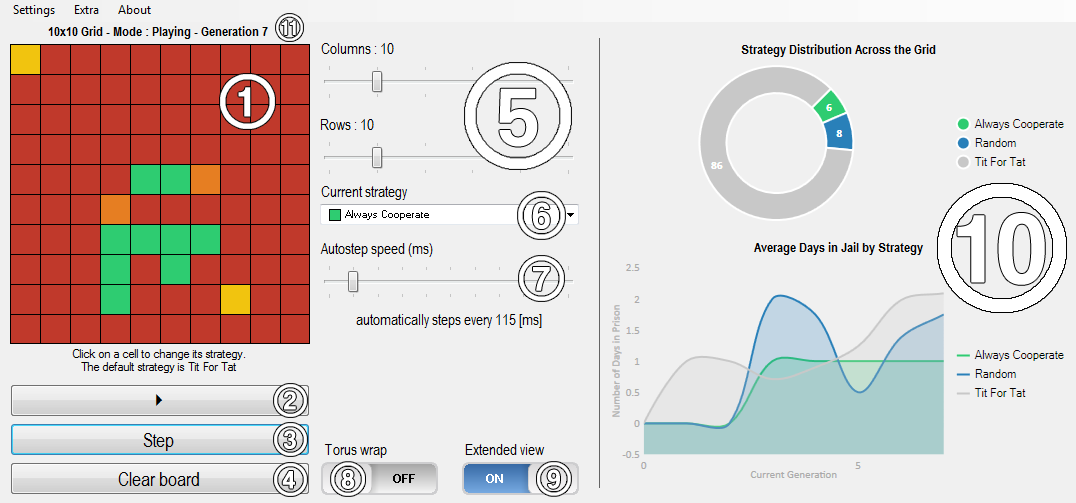
\includegraphics[width=\linewidth]{main_view.png}
    \caption{Fenêtre principale de l'application}
\end{figure}

\vspace{0.25cm}
\begin{description}[labelwidth=4.5cm]
    \small
    \item[\textbf{\textsc{Nom}}] \textbf{\textsc{Description}}
    \vspace{0.1cm}
    \hrule{}
    \item[\texttt{\circled{1} Grille}] : Composant affichant les cellules de l'automate cellulaire.
    \item[\texttt{\circled{2} Play / Pause}] : Démarre ou arrête l'automate cellulaire.
    \item[\texttt{\circled{3} Step}] : Fait avancer d'un temps l'automate cellulaire.
    \item[\texttt{\circled{4} Clear}] : Nettoie le plateau et le remet à son état initial.
    \item[\texttt{\circled{5} Colonnes \& Lignes}] : Change le nombre de colonnes et de lignes de la grille.
    \item[\texttt{\circled{6} Sélection de stratégie}] : Permet la sélection d'une stratégie.
    \item[\texttt{\circled{7} Vitesse}] : Permet d'ajuster la vitesse de l'automate cellulaire en mode automatique.
    \item[\texttt{\circled{8} Switch Torique}] : Permet de basculer entre le mode standard et torique.
    \item[\texttt{\circled{9} Switch vue étendue}] : Permet de basculer entre la vue standard et étendue.
    \item[\texttt{\circled{10} Graphiques}] : Graphiques affichant les données de l'automate cellulaire.
    \item[\texttt{\circled{11} Informations}] : Donne un accès rapide aux informations. (ex : mode d'affichage, taille, etc...)
\end{description}
\hrule{}
\vspace{0.5cm}
\pagebreak

Un menu déroulant se trouvant en haut de la fenêtre permet l'accès aux autres fonctionnalités de l'application tel que la génération de grille ou encore le paramétrage de la matrice des gains.

\begin{figure}[htp]
    \centering
    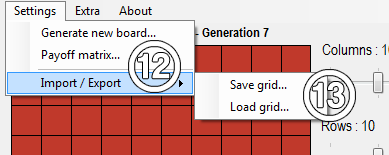
\includegraphics[width=10cm]{main_view_menu.png}
    \caption{Menu déroulant}
\end{figure}

\begin{description}[labelwidth=5cm]
    \small
    \item[\textbf{\textsc{Nom}}] \textbf{\textsc{Description}}
    \vspace{0.1cm}
    \hrule{}
    \item[\texttt{\circled{12} Menu déroulant}] : Composant permettant d'accéder aux autres fonctionnalités
    \item[\texttt{\circled{13} Paramètres d'exportation}] : Permet de sauvegarder la grille actuelle ou d'importer une grille. 
\end{description}
\hrule{}

\subsection{Fonctionnement, fenêtre principale}
\textbf{\circled{1} Grille}

La grille est le composant principal de l'automate cellulaire contenant les différentes cellules. Chaque cellule possède une stratégie pouvant être modifiée à tout moment.

Pour modifier la stratégie d'une cellule, il suffit de sélectionner une stratégie à l'aide du menu déroulant "\tinycircled{6} Sélection de stratégie", puis de cliquer sur l'une des cellules de la grille.

Notez que la grille possède deux modes d'affichage : un mode ou la couleur des cellules représente leur stratégie et un mode ou la couleur des cellules représente leurs actions. Le premier est utilisé lorsque  l'utilisateur modifie la grille, et le deuxième est utilisé en cours de jeu. En cours de jeu, il n'existe que quatre couleurs :

\begin{table}[htp]
\centering
\begin{tabular}{lll}
\cline{1-2}
\textbf{Couleur} & \textbf{Valeur représentée} \\
\cline{1-2}
\tikz \fill [red] (0,0) rectangle (0.2,0.2); Rouge & Cellule ayant trahit les deux derniers tours\\
\tikz \fill [orange] (0,0) rectangle (0.2,0.2); Orange & Cellule coopérante, mais ayant trahi le dernier tour\\
\tikz \fill [yellow] (0,0) rectangle (0.2,0.2); Jaune & Cellule traître, mais ayant coopéré le dernier tour\\
\tikz \fill [green] (0,0) rectangle (0.2,0.2); Vert & Cellule ayant coopéré les deux derniers tours\\
\cline{1-2}
\end{tabular}
\caption{Sens des différentes couleurs en cours de jeu}
\end{table}


Quand on place des stratégies, la couleur représente la stratégie de la cellule. Il existe de nombreuses stratégies, elles ne seront donc pas toutes listées dans ce document. Voici à quoi peut ressembler les stratégies des cellules dans l'application :
\begin{table}[htp]
\centering
\begin{tabular}{lll}
\cline{1-2}
\textbf{Couleur} & \textbf{Valeur représentée} \\
\cline{1-2}
\tikz \fill [gray] (0,0) rectangle (0.2,0.2); Gris & Tit for Tat\\
\tikz \fill [RoyalBlue] (0,0) rectangle (0.2,0.2); Bleu & Random\\
\tikz \fill [RoyalPurple] (0,0) rectangle (0.2,0.2); Violet & Blinker\\
\tikz \fill [orange] (0,0) rectangle (0.2,0.2); Orange & Fortress\\
etc... & etc...\\
\cline{1-2}
\end{tabular}
\caption{Sens des différentes couleurs lors du placement des stratégies}
\end{table}


\textbf{\circled{2} Play / Pause}

Le bouton "\tinycircled{2} Play / Pause" sert à lancer ou à arrêter le mode automatique de l'automate cellulaire. Dans ce mode, l'automate cellulaire avancera automatiquement à une intervalle régulière. Cette intervalle peut être modifiée à l'aide du composant "\tinycircled{7} Vitesse".

Pour démarrer le mode automatique, cliquez sur le bouton {\footnotesize{\faPlay{}}}. Après un clic, le bouton {\footnotesize{\faPlay{}}} se transformera en {\footnotesize{\faPause{}}}, ce qui permet d'arrêter le mode automatique.

\vspace{0.5cm}
\textbf{\circled{3} Step}

Le bouton "\tinycircled{3} Step" permet de faire avancer le jeu du dilemme du prisonnier. A chaque clic du bouton "\tinycircled{3} Step", toutes les cellules jouent une partie du dilemme du prisonnier avec leurs voisins et mettent à jour leur couleur.

Les "\tinycircled{10} Graphiques" sont également mis-à-jour avec de nouvelles valeurs en temps réel à chaque clic du bouton.

\vspace{0.5cm}
\textbf{\circled{4} Clear}

Ce bouton permet de remettre le plateau dans son état initial. Il remplace la stratégie de chaque cellule du plateau par la stratégie par défaut. Il garde cependant les dimensions actuelles de la grille. La stratégie par défaut est indiqué en dessous de la grille.

\vspace{0.5cm}
\textbf{\circled{5} Colonnes \& Lignes}

Les \textit{sliders} pour colonnes et lignes permettent de changer le nombre de cellules de la grilles. Il est possible de créer une grille possédant au minimum cinq lignes ou colonnes et au maximum trente lignes ou colonnes.

Changer le nombre de colonnes et de lignes de la grille efface la totalité du contenu de cette dernière et la remet dans son état initial. Il est donc impératif de sauvegarder une grille (voir "\tinycircled{12} Import et export de données") si nécessaire avant de changer sa taille, le cas échéant entraînant la perte des données actuelles.

\vspace{0.5cm}
\textbf{\circled{6} Sélection de stratégie}

A l'aide du menu déroulant "\tinycircled{6} Sélection de stratégie", il est possible de sélectionner une stratégie à appliquer à une cellule. Le menu déroulant contient la liste de toutes les stratégies disponibles. Pour appliquer une stratégie, on clique simplement sur l'une des cellules de la grille.

Pour plus d'informations sur le remplacement des stratégies des cellules, voir "\tinycircled{1} Grille".

\vspace{0.5cm}
\textbf{\circled{7} Vitesse}

Ce \textit{slider} permet de contrôler la vitesse du mode automatique de l'automate cellulaire (voir "\tinycircled{2} Play / Pause"). Le temps de l'intervalle est directement indiquée en dessous du \textit{slider} et est compté en millisecondes $[ms]$.

\pagebreak
\textbf{\circled{8} Switch Torique}

Le \textit{switch} torique définit le mode d'interaction entre cellules. Il y a actuellement deux modes, un mode par \texttt{défaut} (\texttt{off}) et un mode \texttt{torique} (\texttt{on}). Quand le \textit{switch} est en mode \texttt{torique} (\texttt{on}), les cellules se trouvant en bords de grille sont voisines avec celles se trouvant aux bords opposés comme si la grille était un "tore" (forme géométrique). En mode \texttt{défaut} (\texttt{off}), les voisins d'une cellule se trouvent directement a coté d'elle. La figure ci-dessous représente les différents modes d'inteactions entre cellules :

\begin{figure}[htp]
    \centering
    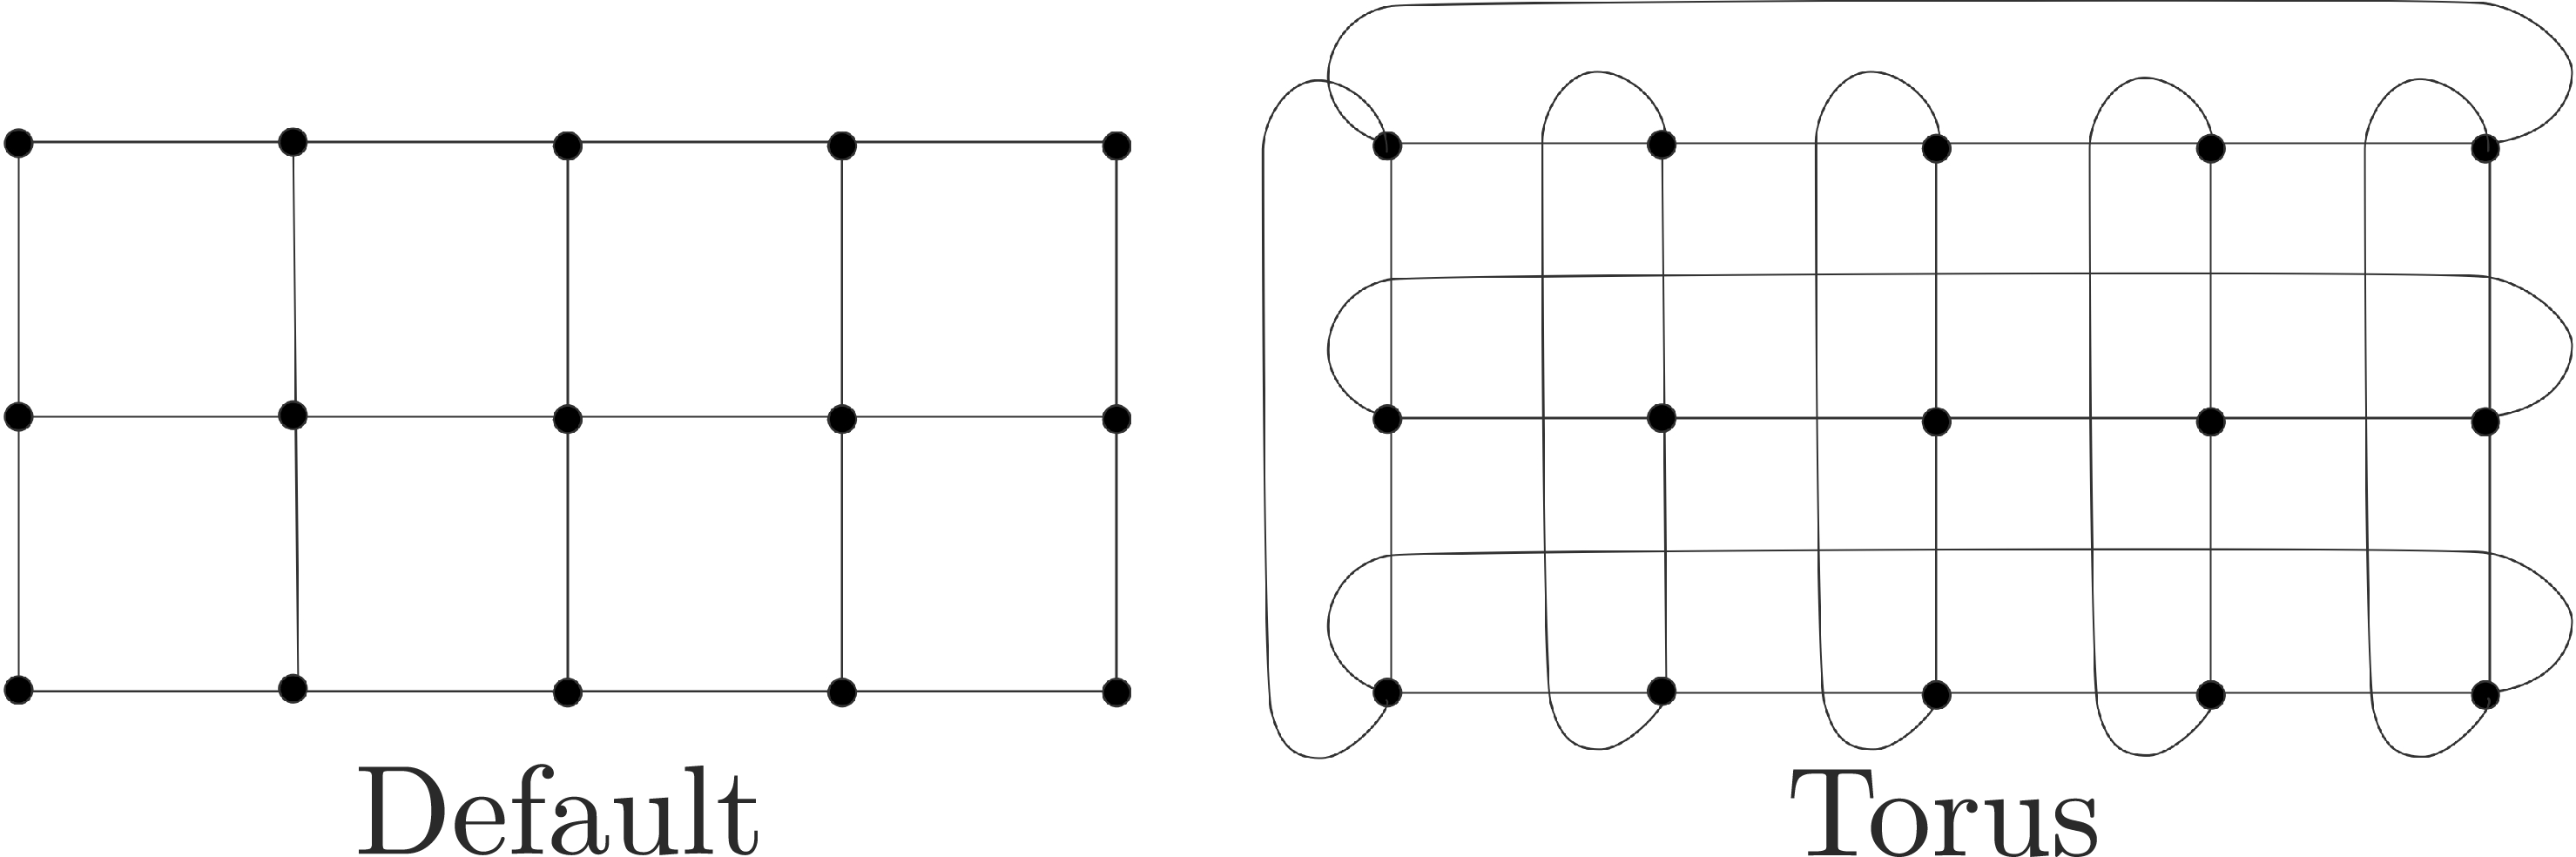
\includegraphics[width=\linewidth]{wrapmode.png}
    \caption{Voisinage des cellules selon le \textit{switch} torique}
\end{figure}


\vspace{0.5cm}
\textbf{\circled{9} Switch vue étendue}

Ce \textit{switch} permet de basculer entre les deux modes de vue de l'application : Le mode normal et le mode étendu. En mode étendu, des graphiques (voir "\tinycircled{10} Graphiques") sont affichés et permettent de visualiser les informations de l'automate cellulaire en temps réel.

\begin{figure}[htp]
    \centering
    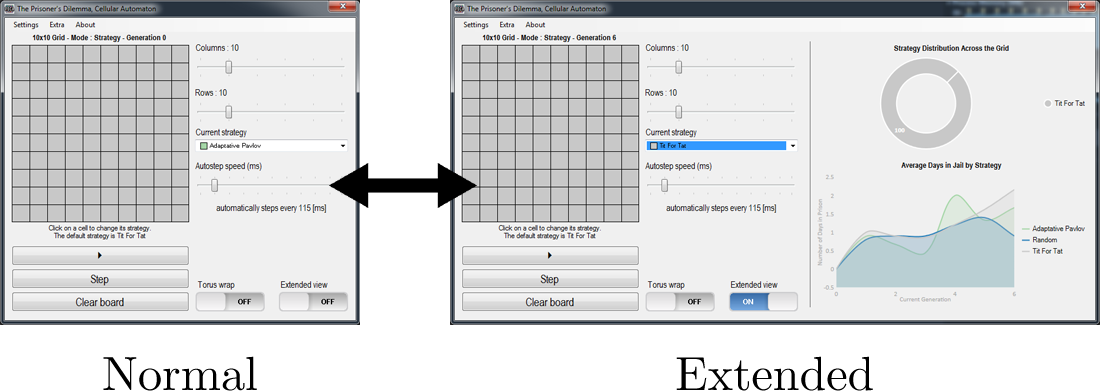
\includegraphics[width=\linewidth]{normal_extended_view.png}
    \caption{Comparaison vue normale et vue étendue}
\end{figure}

\vspace{0.5cm}
\textbf{\circled{10} Graphiques}

Les graphiques sont des composants permettant d'afficher les informations relatives à l'automate cellulaire en temps réel. Les graphiques sont uniquement visibles depuis la vue étendue (voir "\tinycircled{9} Switch vue étendue"). Le graphique supérieur indique la répartition des stratégies sur le plateau, et le graphique inférieur montre le nombre de jours qu'une stratégie passe en prison en moyenne.

\pagebreak
\textbf{\circled{12} Menu déroulant}

Le menu déroulant est un composant donnant l'accès au reste des fonctions de l'application. Comme indiqué sur la figure 2, le menu déroulant donne l'accès aux fonctionnalités suivantes :

\begin{itemize}
    \item Génération de grille
    \item Configuration de la matrice des gains
    \item Importation et exportation de grilles
    \item \textit{Benchmarking} de stratégies
    \item A propos
\end{itemize}

Il suffit de cliquer sur l'une des options du menu pour y accéder.



\vspace{0.5cm}
\textbf{\circled{13} Import et export de données}

Ces options permettent d'exporter ou d'importer une grille au format "\textit{.xml}". Notez que l'on exporte/importe uniquement certaines informations de la grille :

\begin{itemize}
    \item Dimensions de la grille (hauteur, largeur)
    \item Matrice des gains
    \item Cellules et leurs stratégies
\end{itemize}

Toutes informations relatives à une partie en cours ne seront pas sauvegardées.

Pour exporter/importer un fichier "\textit{.xml}", on navigue dans le menu déroulant (voir "\tinycircled{12} Menu déroulant") jusqu'à atteindre l'onglet "Import / Export". Il ne reste plus qu'à cliquer sur l'option désirée et de choisir ou stocker / récupérer le fichier "\textit{.xml}".

\begin{figure}[htp]
    \centering
    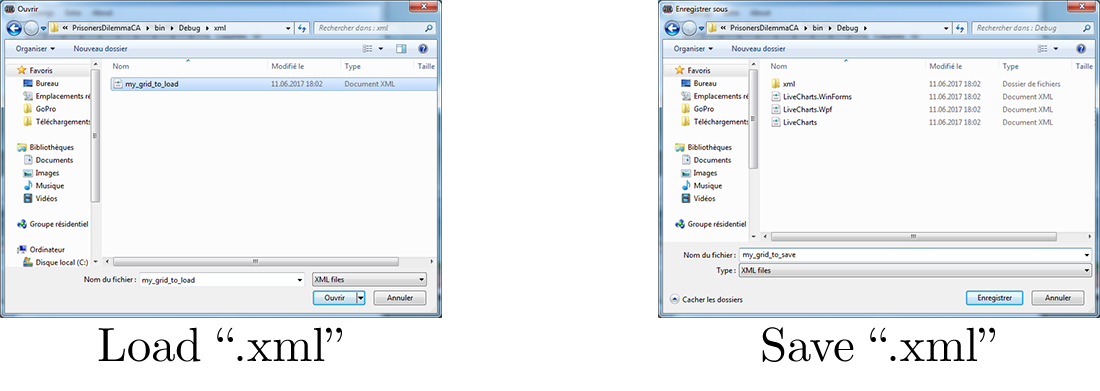
\includegraphics[width=\linewidth]{import_export.png}
    \caption{Importation et exportation au format "\textit{.xml}"}
\end{figure}


\pagebreak
\section{Génération d'un plateau}
L'interface de génération de plateaux sert à créer des grilles de cellules contenant des stratégies réparties aléatoirement. Cependant, il est possible d'avoir un certain contrôle sur la répartition de ces dernières. Il est possible d'ajuster la proportion de chaque stratégie présente sur le plateau à l'aide de différents \textit{sliders}.

\begin{figure}[htp]
    \centering
    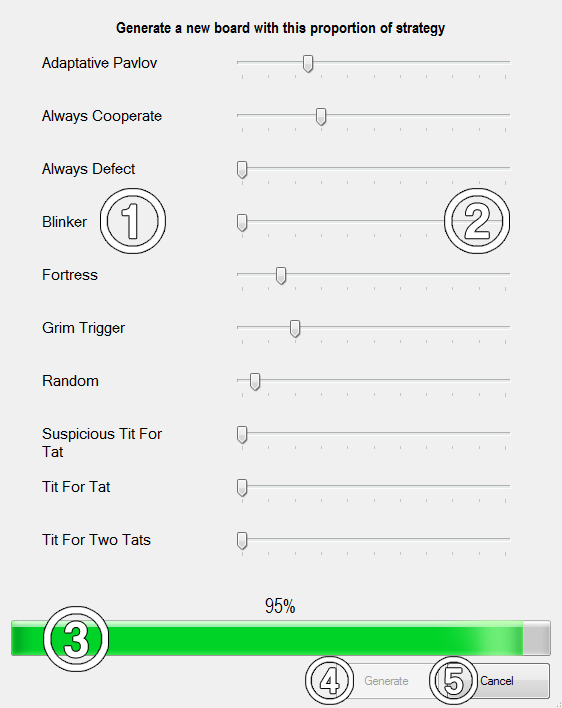
\includegraphics[width=10cm]{generation_view.png}
    \caption{Fenêtre de génération d'un plateau}
\end{figure}

\vspace{0.25cm}
\begin{description}[labelwidth=5cm]
    \small
    \item[\textbf{\textsc{Nom}}] \textbf{\textsc{Description}}
    \vspace{0.1cm}
    \hrule{}
    \item[\texttt{\circled{1} Nom de stratégie}] : Nom de la stratégie à poser sur le plateau.
    \item[\texttt{\circled{2} Pourcentage de stratégie}] : Pourcentage de stratégie à répartir sur le plateau.
    \item[\texttt{\circled{3} Pourcentage total}] : Pourcentage total des stratégies
    \item[\texttt{\circled{4} Valider}] : Valide et lance la génération d'un plateau.
    \item[\texttt{\circled{5} Annuler}] : Annule la génération du plateau.
\end{description}
\hrule{}
\vspace{0.5cm}
\pagebreak{}
\subsection{Fonctionnement, génération d'un plateau}
\textbf{\circled{2} Pourcentage de stratégie}

Le pourcentage de chaque stratégie peut être ajusté à l'aide d'un \textit{slider} allant de 0 à 100. En déplaçant le curseur du \textit{slider}, on peut observer le pourcentage total du plateau augmenter (voir \tinycircled{3} Pourcentage total). Quand le pourcentage total atteint 100\%, la grille est désormais pleine et il est impossible d'incrémenter la valeur de n'importe quel \textit{slider}. Après avoir atteint les 100\%, le bouton \tinycircled{4} Valider s'active et il est possible de l'actionner.

\textbf{\circled{4} Valider}

Le bouton \tinycircled{4} Valider permet de confirmer le choix de l'utilisateur et de lancer la génération de la grille. Ce bouton est uniquement actionnable si le pourcentage affiché est égal à 100\%. Après avoir cliqué sur le bouton, une redirection vers le menu principale est effectuée et la grille générée est affichée.

\pagebreak
\section{Ajustement de la matrice des gains}
\begin{figure}[htp]
    \centering
    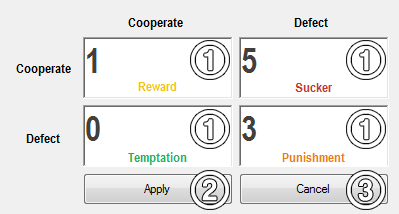
\includegraphics[width=10cm]{payoffmatrix_view.png}
    \caption{Interface d'ajustement de matrice de gains}
\end{figure}

\vspace{0.25cm}
\begin{description}[labelwidth=3cm]
    \small
    \item[\textbf{\textsc{Nom}}] \textbf{\textsc{Description}}
    \vspace{0.1cm}
    \hrule{}
    \item[\texttt{\circled{1} Gains}] : Nombre de jours passés en prison. 
    \item[\texttt{\circled{2} Appliquer}] : Valide la matrice des gains et applique les changements.
    \item[\texttt{\circled{3} Annuler}] : Annule la modification de la matrice de gains.
\end{description}
\hrule{}
\vspace{0.5cm}

\subsection{Fonctionnement, matrice des gains}
\textbf{\circled{1} Gains}

Il existe quatre gains différents dans le dilemme du prisonnier, chacun correspondant à une paire d'actions des joueurs. Voici les noms de ces derniers :

\begin{table}[htp]
    \centering
    \begin{tabular}{lllll}
        \hline
        \textbf{Joueur 1} &   & \textbf{Joueur 2} &               & \textbf{Nom du gain}       \\ \hline
        Coopérer          & + & Coopérer          & $\rightarrow$ & Récompense (reward $R$)    \\
        Trahir            & + & Coopérer          & $\rightarrow$ & Tentation (temptation $T$) \\
        Coopérer          & + & Trahir            & $\rightarrow$ & Duperie (sucker $S$)       \\
        Trahir            & + & Trahir            & $\rightarrow$ & Punition (punishment $P$)  \\ \hline
    \end{tabular}
    \caption{Action des joueurs et gains résultants}
\end{table}

Ces différents gains sont présents dans les quatre cases de l'interface et peuvent être ajustés à tout moment. Cependant, la valeur de ces gains doit être conforme à deux règles :

\begin{framed}
    \centering
    Tentation < Récompense < Punition < Duperie\\
    2 * Récompense < Tentation + Duperie
\end{framed}

La première règle assure que trahir soit toujours supérieur en gain à la récompense de coopérer qui est elle même supérieure à la punition, etc... 

La deuxième règle est uniquement présente dans un dilemme du prisonnier \textit{répété} et assure que coopérer deux fois d'affilée est une meilleure solution que de trahir une fois, puis se faire trahir le tour suivant.

Sans ces deux règle, le jeu n'est pas considéré comme un dilemme du prisonnier répété.

\textbf{\circled{2} Appliquer}

Le bouton "\tinycircled{2} Appliquer" permet de valider les changements effectués à la matrice des gains. Si la matrice des gains est conforme aux règles du dilemme du prisonnier (voir "\tinycircled{1} Gains"), on applique les changements, sinon, on affiche un message indiquant les règles.


\pagebreak
\section{\textit{Benchmark} d'une stratégie}
\begin{figure}[htp]
    \centering
    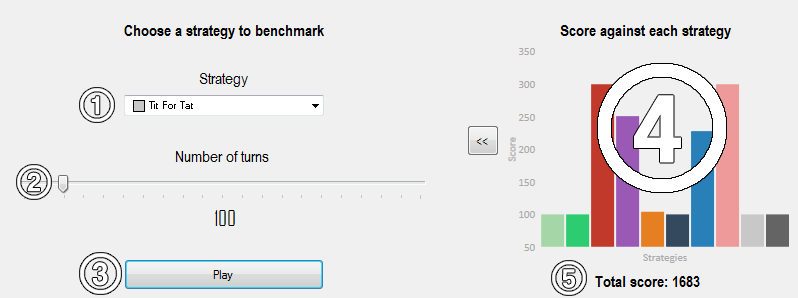
\includegraphics[width=\linewidth]{benchmark_view.png}
    \caption{Fenêtre de benchmark}
\end{figure}

\vspace{0.25cm}
\begin{description}[labelwidth=5cm]
    \small
    \item[\textbf{\textsc{Nom}}] \textbf{\textsc{Description}}
    \vspace{0.1cm}
    \hrule{}
    \item[\texttt{\circled{1} Stratégie sélectionnée}] : Stratégie sélectionnée pour le \textit{benchmark}.
    \item[\texttt{\circled{2} Nombre de tours}] : Nombre de tours de jeu à jouer contre chacune des stratégies.
    \item[\texttt{\circled{3} Lancer la simulation}] : Lance un match contre chacune des stratégies.
    \item[\texttt{\circled{4} Graphique}] : Affiche les résultats détaillés à la fin du match.
    \item[\texttt{\circled{5} Score total}] : Affiche le score total à la fin du match.
\end{description}
\hrule{}
\vspace{0.5cm}

\subsection{Fonctionnement, \textit{benchmark}}
\textbf{\circled{3} Lancer la simulation}

En appuyant sur le bouton "Play", on démarre le \textit{benchmarking} de la stratégie. La stratégie joue ainsi contre toutes les autres stratégies (elle-même inclue) au dilemme du prisonnier autant de fois qu'indiqué par le \textit{slider} "\tinycircled{2} Nombre de tours". Il est important de noter que le \textit{slider} "\tinycircled{2} Nombre de tours" représente le nombre de tours joué contre chaque stratégie et non le nombre de tours total du \textit{benchmarking}.

\textbf{\circled{4} Graphique}

Le graphique permet d'observer les résultats du \textit{benchmarking} sur un histogramme. Chaque colonne représente le score obtenu contre une stratégie et la couleur de cette dernière correspond à la couleur de la stratégie (voir "\tinycircled{1} Grille"). 

Le score total de toutes les parties jouées lors du \textit{benchmark} peut aussi être consulté en dessous du graphique ("\tinycircled{5} Score total").

\pagebreak
\section{Aide intégrée à l'application}
Un manuel utilisateur est intégré dans certaines des vues de l'application. Pour y accéder, il suffit de cliquer sur le bouton "
\includegraphics[height=0.75em]{questionmark.png}" se trouvant en haut à droite des fenêtres concernées.

Voici à quoi ressemble l'une des fenêtre d'aide incluse avec l'application :

\vspace{0.5cm}
\begin{figure}[htp]
    \centering
    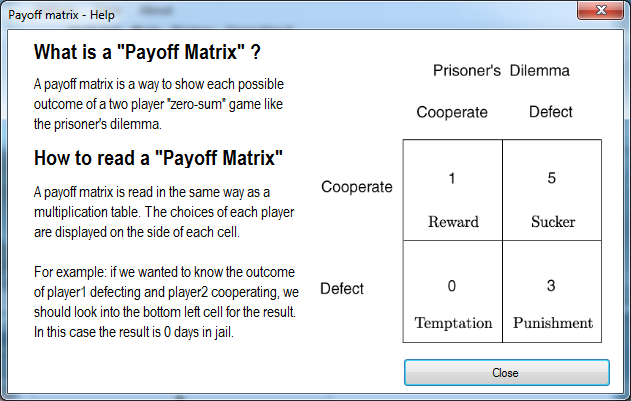
\includegraphics[width=\linewidth - 2cm]{payoff_help.png}
    \caption{Fenêtre d'aide de la matrice des gains}
\end{figure}


\pagebreak
\listoffigures
\listoftables

\end{document}